% This is the aspauthor.tex LaTeX file
% Copyright 2010, Astronomical Society of the Pacific Conference Series

\documentclass[11pt,twoside]{article}
\usepackage{asp2010}
\usepackage{graphicx}



\resetcounters

\bibliographystyle{asp2010}

\markboth{Moins, et al}{ESO Catalogue Facility design and performance}

\begin{document}

\title{ESO Catalogue Facility design and performance}
\author{C. Moins$^1$, J. Retzlaff$^1$, M. Arnaboldi$^1$, S. Zampieri$^1$, N. Delmotte$^1$, V. Forch\'{i}$^1$,
 M. Klein Gebbinck$^1$, J. Lockhart$^1$, A. Micol$^1$, I. Vera Sequeiros$^1$, T. Bierwirth$^1$, M. Peron$^1$, M. Romaniello$^1$, D. Suchar$^1$
\affil{$^1$European Southern Observatory}}

\begin{abstract}
The ESO Phase 3 Catalogue Facility provides investigators with the possibility to ingest catalogues resulting from ESO public surveys and large programs and to query and download their content according to positional and non-positional criteria. It relies on a chain of tools that covers the complete workflow from  submission to validation and ingestion into the ESO archive and catalogue repository and a web application to browse and query catalogues.
This repository consists of two components. One is a Sybase ASE relational database where catalogue meta-data are stored. The second one is a Sybase IQ data warehouse where the content of each catalogue is ingested in a specific table that returns all records matching a user's query. Spatial indexing has been implemented in Sybase IQ to speed up positional queries and relies on the Spherical Geometry Toolkit from the Johns Hopkins University which implements the Hierarchical Triangular Mesh (HTM) algorithm. It is based on a recursive decomposition of the celestial sphere in spherical triangles and the assignment of an index to each of them. It has been complemented with the use of optimized indexes on the non-positional columns that are likely to be frequently used as query constraints.
First tests performed on catalogues such as 2MASS have confirmed that this approach provides a very good level of performance and a smooth user experience that are likely to facilitate the scientific exploitation of catalogues.
\end{abstract}

\section{Overview}
The catalogue facility covers the complete workflow from catalogue submission to data retrieval. The first step is the upload of a catalogue stored in one or several FITS file to a staging area on the ESO's network by a Principal Investigator. After validation, the catalogue is stored in the ESO archive, its meta data is ingested in a Sybase ASE relational database and its content is inserted in a dedicated table on a Sybase IQ data warehouse. Once a catalogue has been published by the operator, ESO users will have the possibility to query catalogues and to download the resulting records in one of the supported format: FITS, TSV, CSV, HTML, VOTABLE. The following picture represents the complete workflow from catalogue submission to querying:
\begin{center}
\setlength\fboxsep{1pt}
\setlength\fboxrule{1pt}
\fbox{
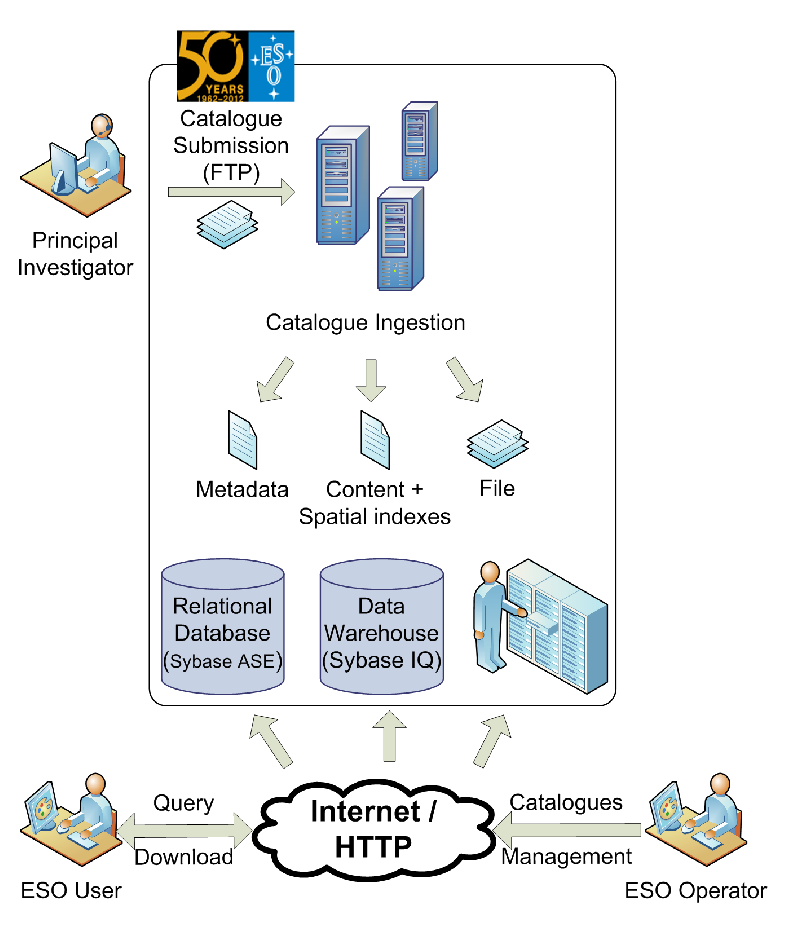
\includegraphics [scale=0.7]{P64_1.eps}
}
\begin{figure}[h]
\caption{Catalogue workflow from submission to web based search}
\end{figure}
\end{center}

\section{Workflow}
\subsection{Catalogue Submission}
Principal investigators of ESO observing programmes return their reduced data products (images, spectra and catalogues) for storage in the ESO archive and subsequent data
publication to the scientific community. This process is called Phase 3 (\citet{phase3} and \citet{messenger})\footnote{http://www.eso.org/sci/observing/phase3.html}.
Catalogues are submitted as FITS files with a primary header containing the catalogue metadata and a BINTABLE extension where the catalogue data are stored. Large catalogues, e.g.
resulting from wide-area surveys, are submitted in the form of multiple FITS files, which are then loaded in the database in order to be published as one seamless catalogue.
The \textit{ESO Science Data Products Standard} \footnote{http://www.eso.org/sci/observing/phase3/p3sdpstd.pdf}
document provides a detailed description of the required structure and data format of reduced data products in order to be accepted and published
by the ESO archive.

\subsection{Catalogue Ingestion}
Catalogues submitted by principal investigators are stored in the ESO archive, their metadata are ingested in a Sybase ASE relational database and their contents are ingested in a Sybase IQ data warehouse. As one of the typical searches includes spatial constraints centered on a point of interest and due to the large number of entries (up to a few billions), spatial indexing has been implemented using the \textit{Spherical Geometry Toolkit} (\citet{spherical})
based on the \textit{Hierarchical Triangular Mesh} (HTM) algorithm. HTM divides recursively the celestial sphere into spherical triangles of roughly equal areas and assigns to each of them a unique integer number (HTM \textit{index}). The \textit{depth} of the HTM index denotes the number of recursions (depth 0 corresponds to the whole sphere), and the number of HTM triangles (or \textit{trixels}) $N$ at a given depth $d>0$ is given by $N(d) = 8\times{4^{d-1}}$. We use depth 20 (the default) which we consider a good compromise between resolution and performance.\\
Upon ingestion, the HTM index corresponding to the coordinates of each object is computed and inserted in a dedicated column of the catalogue table, together with the cartesian coordinates of the corresponding unit vectors. The HTM column is indexed in Sybase IQ with an \textit{High Group Index} optimized for high cardinality data. At query time, the spatial constraint (cone or box search) provided by the archive user is converted to a set of HTM index ranges covering the specified region. To avoid creating too many ranges, which could negatively affect the query performance, the Spherical Toolkit merges neighbouring intervals, introducing an overshoot which is well visible in Figure 2. Therefore we need to complement the HTM condition with the exact geometrical constraint based on the \textit{dot product} in cartesian coordinates to get a more accurate result: the dot product condition for a cone search is $\vec{p}\cdot\vec{c}>cos(\alpha)$, where $\vec{c}$ is the unit vector pointing at the search center, $\vec{p}$ the unit vector of the catalogue objects we are looking for and $\alpha$ denotes the maximum angular distance from the target position, i.e. the radius. The box search requires four dot product conditions, one for each side of the box. The figure below represents the result of a cone search with and without dot product condition:\\

\begin {center}
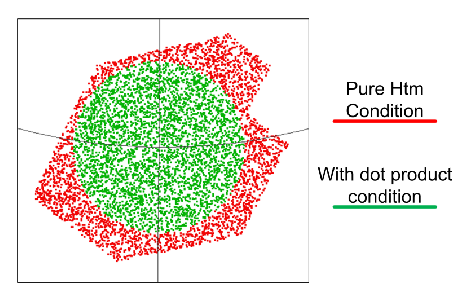
\includegraphics  [scale=0.8]{P64_2}
\begin{figure} [h]
\caption{cone search with and without dot product}
\end{figure}
\end {center}

\subsection{Catalogue Query and Download}
The Catalogue Query Interface is a web application that enables users to:
\begin{itemize}
\item browse the catalogue directory to select the catalogue of interest for viewing its medatadata, querying the catalogue content or
requesting the entire data set from the ESO Archive.
\item define query constraints to search the selected catalogue, including associated catalogues when available, around a single or multiple targets using either a circular region (Cone) or a square (Box). This spatial search can be complemented with constraints on non spatial parameters (e.g. color or magnitude). When a user launches a query, an SQL query is generated on the server side where the spatial condition is represented by a HTM condition generated by the Spherical Geometry Toolkit.
\item display a subset of a query result using an interactive viewer for tabular data (max. 1000 rows) and download the complete result set in one of the supported format: 
FITS, TSV, CSV, VOTable and HTML.
\end{itemize}

\subsection{Performance}
The query performance was measured by executing several searches in different regions of the sky on the 2MASS point source catalogue. Pure spatial queries are fast, thanks to the optimized spatial indexing based on HTM and Sybase IQ. For example a 2 degree cone search selecting hundreds of thousands sources (but retrieving only the first 1000) takes on average 2.6 seconds. Adding non-spatial constraints slows down the query but the performance is still quite good.

\begin{table}[!ht]
\caption{2MASS search results}
\begin{center}
{\small
\begin{tabular}{cccc}
\tableline
\noalign{\smallskip}
Radius & Average number of rows & Average Time (sec) & Non-spatial constraint \\
\noalign{\smallskip}
\tableline
\noalign{\smallskip}
2 arcsec & 0 & 0.179 & no \\
2 deg & 175045.6 & 2.65 & no \\
20 deg & 16264352 & 46.45 & no \\
2 deg & 4366 & 13.1 & yes \\
\noalign{\smallskip}
\tableline
\end{tabular}
}
\end{center}
\end{table}

\section{Conclusion}
The ESO Catalogue Facility provides a reliable and flexible environment that allows a quick ingestion and publication of catalogues. The combination of a Sybase IQ data warehouse, spatial indexing and optimized indexes allows to reach a very good level of performance when querying catalogues, which guarantees a smooth user experience. The Query Interface offers a user friendly access to ESO catalogues that facilitates their scientific exploitation.

\bibliography{P64}

\end{document}
